\documentclass{beamer}

\usetheme{simple}

\usepackage{caption}
\usepackage{xcolor}
\usepackage{fancyvrb}
\usepackage{ulem}
\usetikzlibrary{positioning,calc,automata}

\title{CSC363 Tutorial \#2}
\subtitle{Turing machines and stuff}
\date{January 26, 2022}
\institute{}

\newcommand{\N}{\mathbb N}

\begin{document}

\maketitle

\begin{frame}{Learning objectives this tutorial}
\begin{itemize}
\item Prove that some functions are primitive recursive.
\item Prove more functions are primitive recursive.
\item Talk about ``computable sets''.
\end{itemize}
\end{frame}

\begin{frame}{A bit about myself?}
Hi! I'm some 4th year student studying math/cs. I was sick last week ;w;
\begin{itemize}
    \item Contact: p\textcolor{red}{o}l.zhang@utoronto.ca, or if you prefer Discord, sjorv\#0943
    \item Hobbies: Gaming, taking naps at inappropriate times
    \begin{figure}
        \centering
        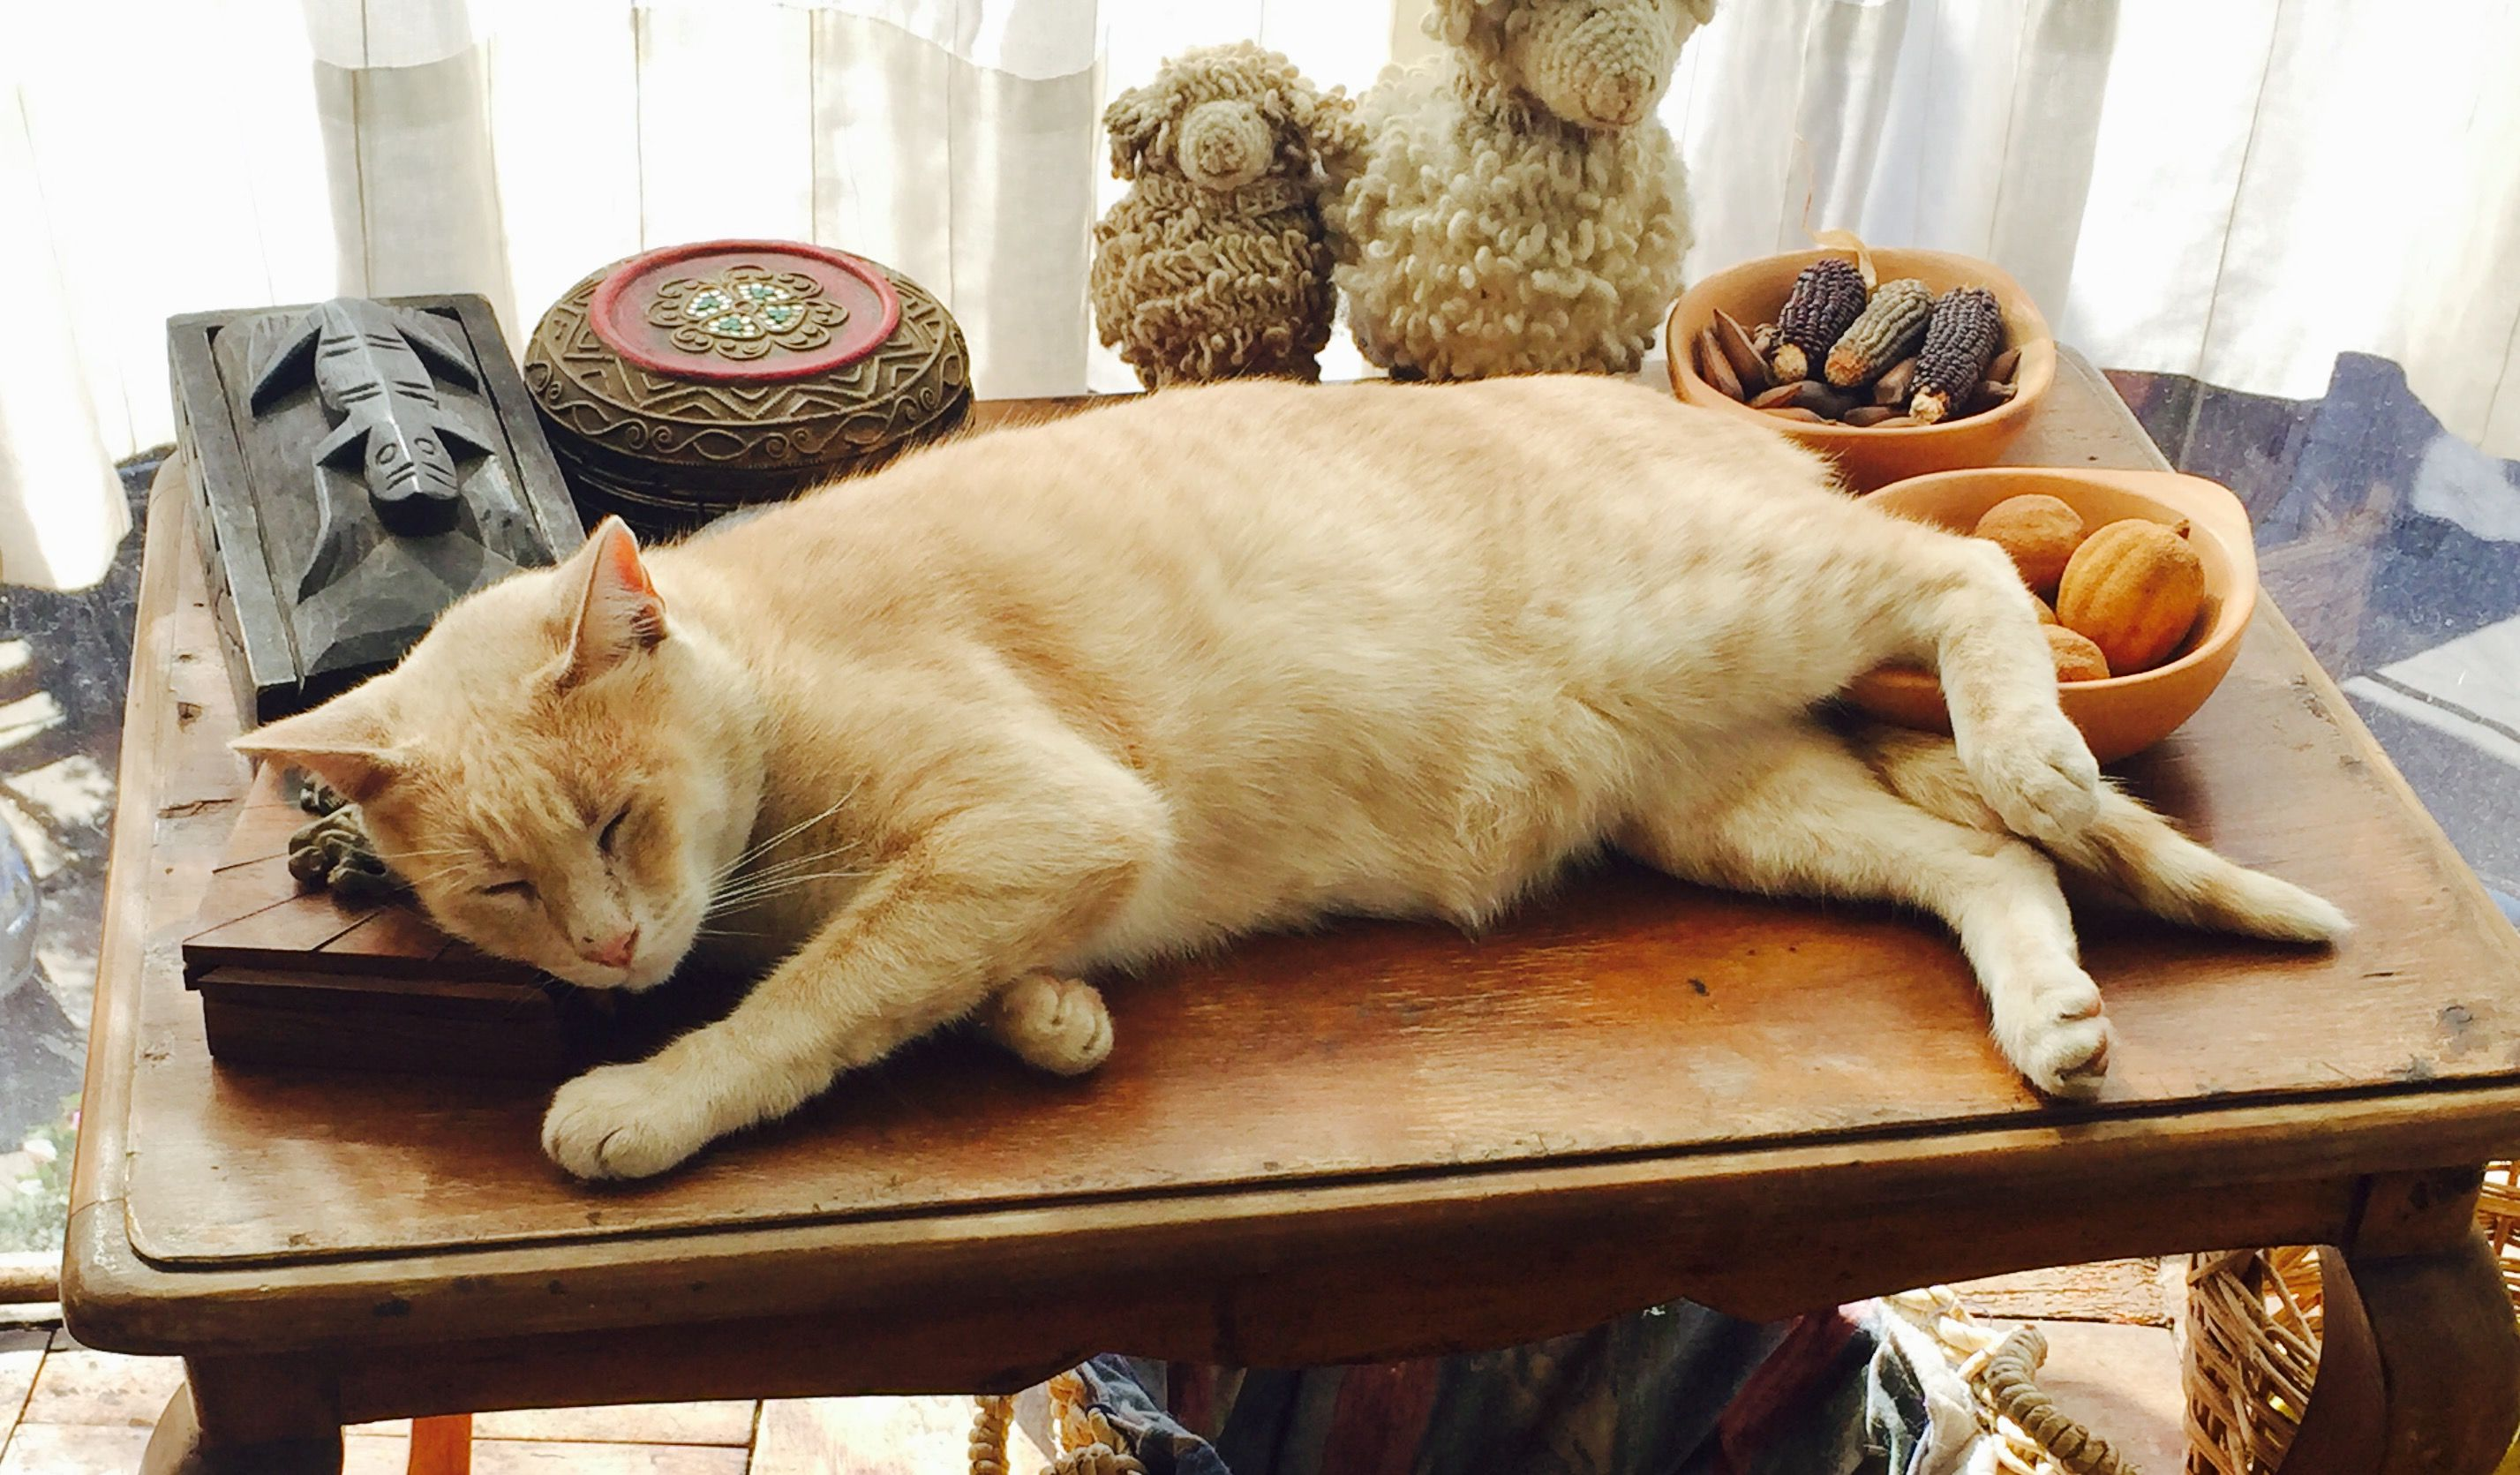
\includegraphics[width=6cm]{img/siesta.jpg}
        \caption*{Not my cat. Cats are cute though.}
    \end{figure}
    \item Favourite food: sushi juice
    \item Office hours: 1-2pm Friday
    \item Website (you can find tutorial slides there): sjorv.github.io
\end{itemize}
\end{frame}

\begin{frame}{PRIM}
\textbf{Question}: What does PRIM stand for?

\pause

\textbf{Question}: What are the initial functions in PRIM?
\end{frame}

\begin{frame}{PRIM}
Recall that PRIM is a set of functions from $\N^k$ to $\N$, intuitively meant to capture what a ``computable'' function is.

\begin{figure}
    \centering
    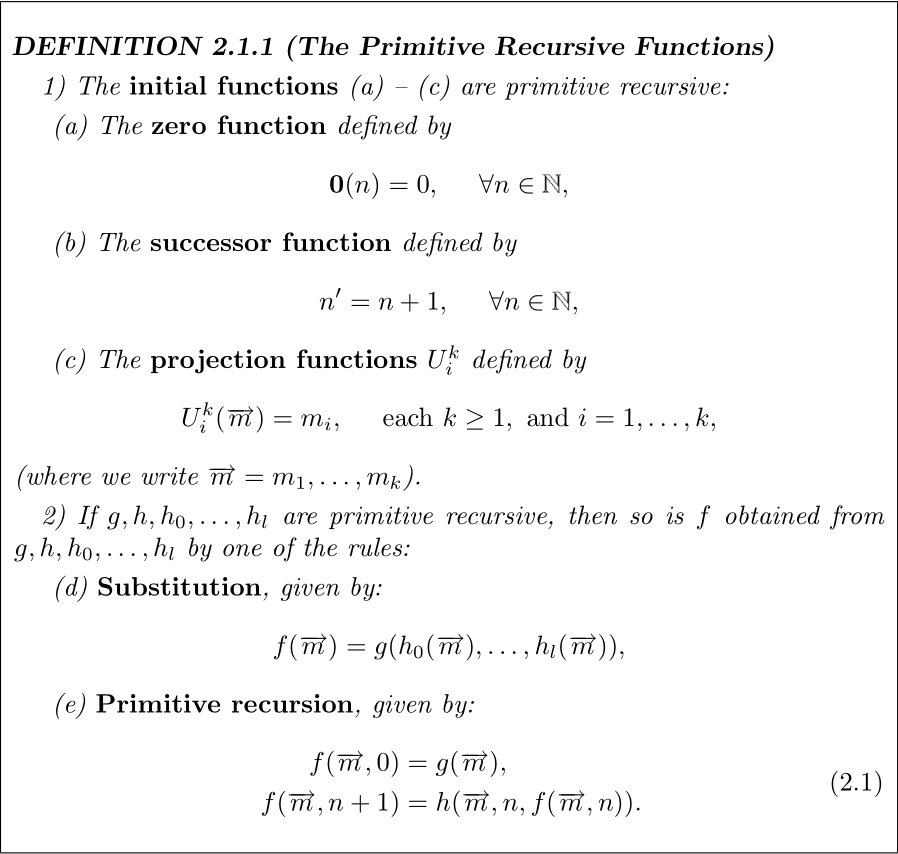
\includegraphics[height=6.5cm]{img/prim_def.png}
    \caption*{Keep this definition handy!}
\end{figure}
\end{frame}

\begin{frame}{Constant functions are in prim}
\textbf{Task}: Prove that $f_k: \N \to \N$, given by $f_k(n) = k$ for all $n \in \N$, is primitive recursive. \pause

\textbf{Ans}: We know $\mathbf 0$ (the zero function) and $S$ (the successor function) are primitive recursive, from (a) and (b). Thus repeatedly applying the substitution rule (d),
$$f_k(n) = \underbrace{S(S(\ldots(S(}_{\text{$k$ times}}\mathbf 0(n)))\ldots))$$
is primitive recursive.
\end{frame}

\begin{frame}{Addition is in prim}
Recall from Lecture 2: the addition function $+: \N^2 \to \N$, $+(m, n) = m + n$, is in PRIM.

\pause

\textbf{Informal Proof}:
$$+(x, 0) = x,$$
$$+(x, n + 1) = S(+(x, n))$$
so using the rule of primitive recursion (e), $+$ is primitive recursive.

\pause

\textbf{Formal Proof}:
We have
$$+(x, 0) = P_1^1(x),$$
$$+(x, n + 1) = g(x, n, +(x, n))$$
where $g(a, b, c) = S(P_3^3(a, b, c))$ is primitive recursive by the substitution rule.
\end{frame}

\begin{frame}{Multiplication is in PRIM}
\textbf{Task}: Now that we know $+$ is in PRIM, prove that the multiplication function $\times: \N^2 \to \N$, $\times(m, n) = mn$, is in PRIM.

\pause

\textbf{Informal Proof}:
$$\times(x, 0) = 0,$$
$$\times(x, n + 1) = +(\times(x, n), x)$$
so using the rule of primitive recursion (e), $\times$ is primitive recursive.

\textbf{Formal Proof}:
We have
$$\times(x, 0) = \mathbf 0(x),$$
$$\times(x, n + 1) = g(x, n, \times(x, n))$$
where $g(a, b, c) = +(P_1^3(a, b, c), P_3^3(a, b, c))$ is primitive recursive by the substitution rule, since we've proven $+$ is primitive recursive.
\end{frame}

\begin{frame}{``Subtraction'' is in PRIM}
\textbf{Task}: Show that $\delta: \N \to \N$, $\delta(n) = \begin{cases} n - 1 & n \geq 1\\ 0 & n = 0\end{cases}$ is in PRIM. 

Hint: Define $f(x, n) = n - 1$ (basically ignoring the first parameter). If we show $f$ is primitive recursive, then $\delta(n) = f(n, n)$ is primitive recursive by the substitution rule.

\pause

\textbf{Proof}: 
Define $f$ as in the hint. We have
$$f(x, 0) = \mathbf 0(x),$$
$$f(x, n + 1) = P_2^3(x, n, f(x, n)) \quad (=n)$$
so $f$ is primitive recursive. Thus $\delta(n) = f(n, n)$ is primitive recursive by substitution rule.
\end{frame}

\begin{frame}{``Subtraction'' is in PRIM}
Unfortunately, we can't define actual subtraction as a function from $\N^2$ to $\N$! We are only allowed to output natural numbers :(

\pause

\textbf{Task}: Show that $\dot{-}: \N^2 \to \N$, $\dot{-}(x, y) = \begin{cases} x - y & x \geq y\\ 0 & x < y\end{cases}$ is primitive recursive.

Hint: primitive recursion, using $\delta$ from before!

\pause

\textbf{Proof}:
We have
$$\dot{-}(x, 0) = P_1^1(x),$$
$$\dot{-}(x, n + 1) = \delta(\dot{-}(x, n))$$
so $\dot{-}$ is primitive recursive.

\tiny{we're being a little informal here! but hopefully you can translate this into a ``formal proof'' as before.}
\end{frame}

\begin{frame}{What is in PRIM?}
So far, we've shown the following are in PRIM:
\begin{itemize}
    \item Any constant function $f_k$.
    \item Addition, multiplication.
    \item ``Subtraction'' (which doesn't go below zero, to make $\N$ happy).
\end{itemize}
\pause
What about the following functions?
\begin{itemize}
    \item Absolute difference $(x, y) \mapsto |x - y|$. \pause
    \item The ``is zero?'' function (inverse sign function): $$\overline{\mathrm{sg}}(x) = \begin{cases}
    1 & x = 0\\
    0 & x \neq 0.
    \end{cases}$$\pause
    \item The ``is not zero'' function (sign function): 
    $$\mathrm{sg}(x) = \begin{cases}
    0 & x = 0\\
    1 & x \neq 0.
    \end{cases}$$\pause
\end{itemize}
They are all primitive recursive!

\end{frame}

\begin{frame}{\color{red}DISCLAIMER!!!!}

I'm about to lie to you.

\color{red}

In our upcoming definition of a ``computable set'', we only assume PRIM functions are ``computable''. This is not true! There are functions not in PRIM that are also computable, such as the Ackermann function.

\pause

So in reality, there are computable sets out there that don't fit our definition of ``computable set''. Explaining this will require week 3 lecture material...

\pause

Either way, every ``computable set'' from our definition will turn out to be ``computable'' in the actual definition.

\end{frame}

\begin{frame}{Computable sets}

Consider $S \subseteq \N$. How do we define the statement ``$S$ is computable'', in terms of primitive recursion?

\pause
A natural way would be to define ``$S$ is computable'' by looking at its \textit{characteristic function} $\chi_S: \N \to \N$, given by
$$\chi_S(n) = \begin{cases}
0 & n \notin S\\
1 & n \in S.
\end{cases}$$

\textbf{Definition}: A set $S \subseteq \N$ is \textit{computable} when its characteristic function $\chi_S$ is primitive recursive.\footnote{I am lying to you here! The actual definition uses ``recursive'' instead of ``primitive recursive'', and ``recursive'' constitutes a larger class of functions. You'll learn (or have learned) about it in this week's lecture.}

\textbf{Task}: Show that the empty set is computable. \pause

\textbf{Ans}: The empty set's characteristic function is just the zero function, which is primitive recursive.
    
\end{frame}

\begin{frame}{Computable sets}

\textbf{Task}: Show that the singleton set $\{0\}$ is computable. \pause

\textbf{Ans}: The characteristic function of $\{0\}$ is just the inverse sign function
$$\overline{\mathrm{sg}}(x) = \begin{cases}
    1 & x = 0\\
    0 & x \neq 0.
    \end{cases}$$
which, as we have shown, is computable.
    
\end{frame}

\begin{frame}{Computable sets}

\textbf{Task}: Show that any singleton set $\{k\}$, with $k \in \N$ is computable. \pause

\textbf{Ans}: The absolute difference $(x, y) \mapsto |x - y|$ is primitive recursive. Thus
$$\overline{\mathrm{sg}}(|x - k|) = \begin{cases}
1 & x = k\\
0 & x \neq k
\end{cases}$$
is primitive recursive. But this is just the characteristic function of $\{k\}$!
    
\end{frame}

\begin{frame}{Computable sets}

\textbf{Task}: Show that any \textit{finite} set $\{k_1, \ldots, k_m\}$, with $k_1, \ldots, k_m \in \N$, is computable. \pause

\textbf{Ans}: What if we added the indicator functions of each singleton set $\{k_1\}, \ldots, \{k_m\}$? Notice that
$$
\overline{\mathrm{sg}}(|x - k_1|) + \ldots + \overline{\mathrm{sg}}(|x - k_m|) > 0 
$$
if and only if $x$ is in $\{k_1, \ldots, k_m\}$. Thus
$$
\mathrm{sg}(\overline{\mathrm{sg}}(|x - k_1|) + \ldots + \overline{\mathrm{sg}}(|x - k_m|)) = 1
$$
if and only if $x$ is in $\{k_1, \ldots, k_m\}$, so our characteristic function is primitive recursive.
    
\end{frame}

\begin{frame}{Computable sets}

\textbf{Task}: Suppose $S_1, S_2 \subseteq \N$ are both computable. Show that $S_1 \cup S_2$ is computable. \pause

\textbf{Ans}: Add the indicator functions!
$$
\mathrm{sg}(\chi_{S_1}(x) + \chi_{S_2}(x)) = 1
$$
if and only if $x$ is in $S_1$ or $x$ is in $S_2$, so our characteristic function is primitive recursive.
    
\end{frame}

\begin{frame}{Computable sets}

What other sets are computable?
\begin{itemize}
    \item The even numbers $\{0, 2, 4, \ldots\}$. (Prove the remainder function $(x, y) \mapsto x \% y$ is in PRIM!)
    \item The prime numbers.
    \item Pretty much every set that ever comes up in number theory!
\end{itemize}
\end{frame}


\begin{frame}{What's this all about?}
We're trying to build a mathematical definition of ``computable'', from multiple different perspectives:
\begin{itemize}
    \item Computation with Turing machines; \pause
    \item Computation with URMs (briefly); \pause
    \item Computation with primitive recursive functions; \pause
    \item \sout{Computation with Lambda Calculus} Oh no! We're not gonna cover this unfortunately :(\footnote{Unless the curriculum changes, that is.}\pause
\end{itemize}
These all turn out to give an ``equivalent'' definition of what is computable. Fundamentally, there are things that computers cannot do, regardless of the framework of computation we use!


Primitive recursion is probably the most ``abstract'' and thus the hardest to grasp intuitively, but it is worthwhile from a historical perspective.
\end{frame}








\end{document}